\documentclass[11pt]{article}
\usepackage[margin=0.8in]{geometry}
\usepackage{lmodern,microtype,xurl,booktabs,graphicx,amsmath,amssymb,xcolor,hyperref}
\hypersetup{colorlinks=true,urlcolor=blue,linkcolor=blue,pdftitle={Check the evidence before reporting a research-data link as broken},pdfauthor={James N. Jean IV}}
\setlength{\parindent}{0pt}\setlength{\parskip}{6pt}
\newcommand{\MSourceItems}{100}
\newcommand{\MCandidates}{72}
\newcommand{\MLookups}{16}
\newcommand{\MRealPairs}{16}
\newcommand{\MControls}{6}
\newcommand{\MSourceFiles}{17}
\newcommand{\MNativeChecks}{346}
\newcommand{\MDevChecks}{741}
\newcommand{\MFinalChecks}{760}
\newcommand{\MDeps}{37}
\newcommand{\MCaptureBytes}{922,142}
\newcommand{\MFigureValues}{64}
\newcommand{\MCoordinates}{248}
\newcommand{\MDevReal}{8}
\newcommand{\MDevControls}{3}
\newcommand{\MDevNaiveAlerts}{3}
\newcommand{\MDevReviewCandidates}{3}
\newcommand{\MDevNaiveFalse}{0}
\newcommand{\MDevConservativeFalse}{0}
\newcommand{\MDevUnknown}{8}
\newcommand{\MDevRepeatMin}{1227.678}
\newcommand{\MDevRepeatMax}{1229.131}
\newcommand{\MDevReferenceMin}{177.387}
\newcommand{\MDevReferenceMax}{259.678}
\newcommand{\MFinalReal}{8}
\newcommand{\MFinalControls}{3}
\newcommand{\MFinalNaiveAlerts}{3}
\newcommand{\MFinalReviewCandidates}{3}
\newcommand{\MFinalNaiveFalse}{0}
\newcommand{\MFinalConservativeFalse}{0}
\newcommand{\MFinalUnknown}{8}
\newcommand{\MFinalRepeatMin}{1231.938}
\newcommand{\MFinalRepeatMax}{1233.746}
\newcommand{\MFinalReferenceMin}{114.356}
\newcommand{\MFinalReferenceMax}{158.980}
\newcommand{\MObservedItems}{22}
\newcommand{\MObservations}{44}
\newcommand{\MRequestSteps}{76}
\newcommand{\MRealResponses}{32}
\newcommand{\MControlResponses}{12}
\newcommand{\MExactGETStarts}{57}
\begin{document}
\begin{center}
{\LARGE\bfseries Check the evidence before reporting\\a research-data link as broken}\par
\vspace{8pt}James N. Jean IV\\
Independent research and implementation study\quad 30 October 2026\\
{\small Bounded observation benchmark, not peer reviewed}
\end{center}
\section*{Decision brief}
A research library maintainer needs an honest review queue. An unsuccessful request can be an access or transport problem; an accepted request can still return no usable content. This study compares two fixed response-triage rules and releases an offline exercise that retains those distinctions.

The bounded source cohort has \MRealPairs{} real dataset DOIs and \MControls{} authored controls. In each phase, both rules flag the same three controls and have zero apparent false alerts among eight available browser references. There is \textbf{no observed false-alert reduction}. The conservative rule leaves the eight real links per phase unknown after repeated empty HTTP 202 responses, rather than certifying file access.

\begin{center}\begin{tabular}{lrr}\toprule
Observed conditional result & Development & Final\\\midrule
Available real browser references & \MDevReal & \MFinalReal\\
Authored not-found controls & \MDevControls & \MFinalControls\\
Naive broken alerts & \MDevNaiveAlerts & \MFinalNaiveAlerts\\
Conservative DOI review candidates & \MDevReviewCandidates & \MFinalReviewCandidates\\
Apparent false alerts, naive & \MDevNaiveFalse & \MFinalNaiveFalse\\
Apparent false alerts, conservative & \MDevConservativeFalse & \MFinalConservativeFalse\\
Conservative real-link unknowns & \MDevUnknown & \MFinalUnknown\\\bottomrule
\end{tabular}\end{center}

\textbf{Practical recommendation.} Retain reasons, times and unavailable states. Two spaced not-found responses can justify checking DOI routing and metadata; they do not prove permanent data loss. Keep a visible matching landing page separate from verified file access and scientific validity.

\textbf{Evidence boundary.} All real items are Karger Figshare datasets in one conditional metadata slice. Browser references are later agent inspections without independent human adjudication. Controls are invented identifiers, not discovered broken scholarly links. Population error rates, actual workload savings, automatic repair and source-file availability are unmeasured.
\newpage
\section*{1. A fixed metadata cohort}
One Crossref response retrieves \MSourceItems{} journal-article records from the fixed 2019 publication-date query with DOI supplement relations. Qualifying relation entries produce \MCandidates{} candidate parent/target pairs. Assertion provenance is retained; deposited relationships do not prove that data substantively support a paper's claims.

Eligible prefixes are 10.5061, 10.6084 and 10.5281. Qualification requires a public DataCite Findable record with general resource type Dataset, with a forty-lookup ceiling. The first \MRealPairs{} lexicographically ordered pairs with distinct parent and target DOIs qualify in \MLookups{} lookups. Alternating pairs assign eight real datasets per phase. All selected targets actually use prefix 10.6084 and Karger Figshare. The other allowed families are not evaluated platforms.

Three fixed authored DOI controls are added per phase, without real parent-article allegations. Observed matching DOI Not Found pages establish their local reference state. Their invented syntax alone does not supply a label. Syntax-invalid cases remain fixtures.

Crossref permits metadata reuse with separate abstract rights, and DataCite describes public metadata as CC0. Complete metadata responses, browser DOM and HTTP originals remain private. Public fields contain minimal DOI/relationship facts, sanitized states, times and hashes. No raw dataset, abstract or third-party manuscript is redistributed.

\MSourceFiles{} exact metadata response entities are preserved. Independent DuckDB JSON/SQL checks the facts and identity ledger in \MNativeChecks{} conditions. Hashes identify local decoded entities, not publisher checksums. A public metadata 404 would not establish that a DOI was never registered, and Findable metadata do not establish a working file download.

An earlier metadata-only count preflight returned a rate limit on its immediate second request. It remains preserved and did not label a source missing. The query was fixed before landing outcomes. This current, Findable-conditioned slice is not a publication-year liveness forecast or original-vintage availability study.
\newpage
\section*{2. Observe the response without inventing availability}
Each of \MObservedItems{} items is observed twice, giving \MObservations{} observations and \MRequestSteps{} request steps. The collector uses allowlisted public HTTPS landing routes, at most five redirects, a 256 KiB terminal-HTML bound and a twenty-minute phase-wide repeat guard. Authentication, file endpoints, private/literal addresses, unsupported redirects and denied access are guarded. Saved source captures, receipts and DOM total \MCaptureBytes{} bytes, below 100 MiB. Automatic browser preview traffic is not audited.

\begin{center}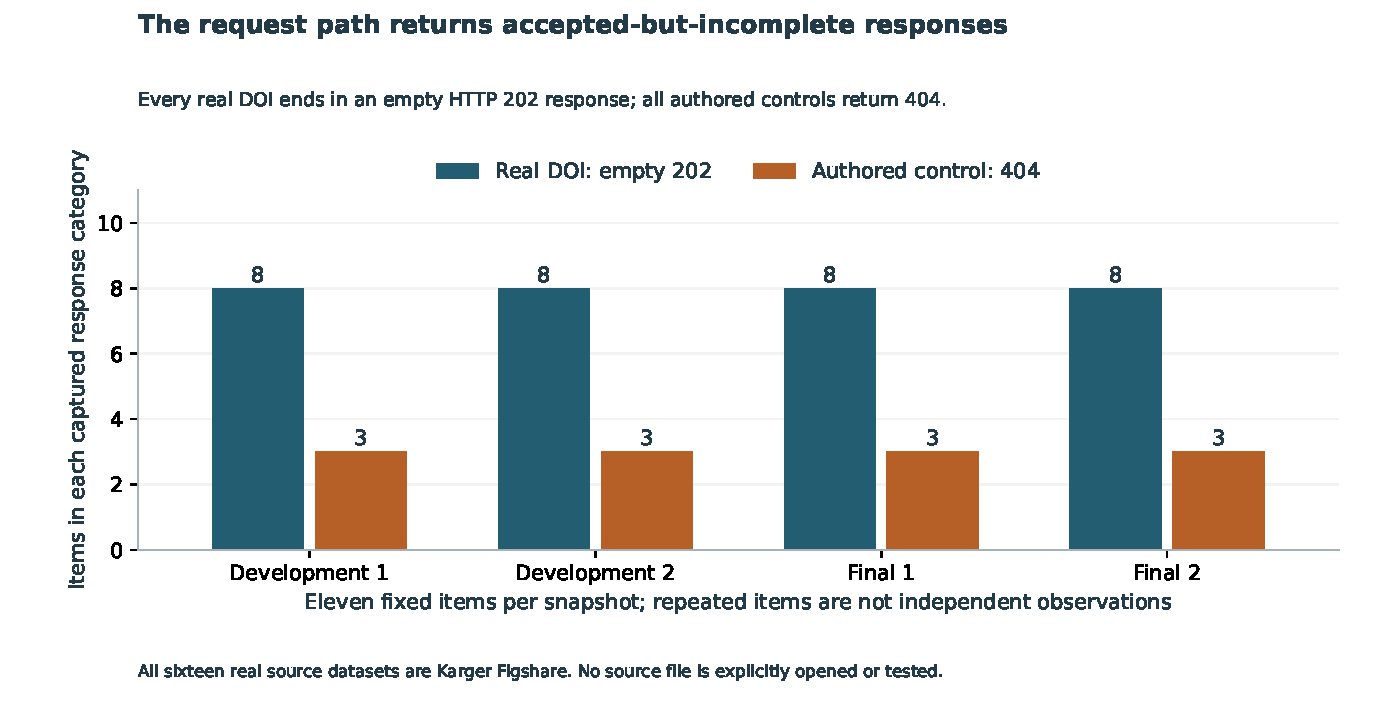
\includegraphics[width=\linewidth]{images/captured_responses.pdf}\end{center}

All \MRealResponses{} real-item observations finish with HTTP 202 and zero stored terminal-body bytes; all \MControlResponses{} control observations finish with 404. RFC 9110 describes 202 as accepted without completed processing. This records a response class, without inferring an underlying job, security mechanism or service cause. Browser pages visibly match dataset identities and show Download controls. No download was explicitly opened; file availability remains untested.

The first development step-start time includes DNS/preparation and courtesy delay; exact GET initiation was not separately logged. Later captures log it, for \MExactGETStarts{} request steps. Actual completion timestamps enforce the repeat gate. Initial protocol language treated successful 2xx broadly; a native binding clarified 202/204 semantics after the first development observations and before comparison/final probes, preserving original responses.
\newpage
\section*{3. Fixed rules and the negative comparison}
The authored naive rule emits a broken alert for a first observed non-2xx terminal response or transport failure. Never-requested items remain unknown. Conservative triage suggests DOI review only after two valid uncensored 404/410 responses at least twenty minutes apart. Other access, rate, transport, server or incomplete-response states remain unknown. Neither rule verifies files.

No model is trained, probability calibrated, threshold optimized or waiting interval empirically selected. Interval and cohort size are authored bounds. The alerts have different meanings: a naive broken assertion is stronger than a suggestion to inspect DOI routing. Their counts cannot become measured workload savings.

\begin{center}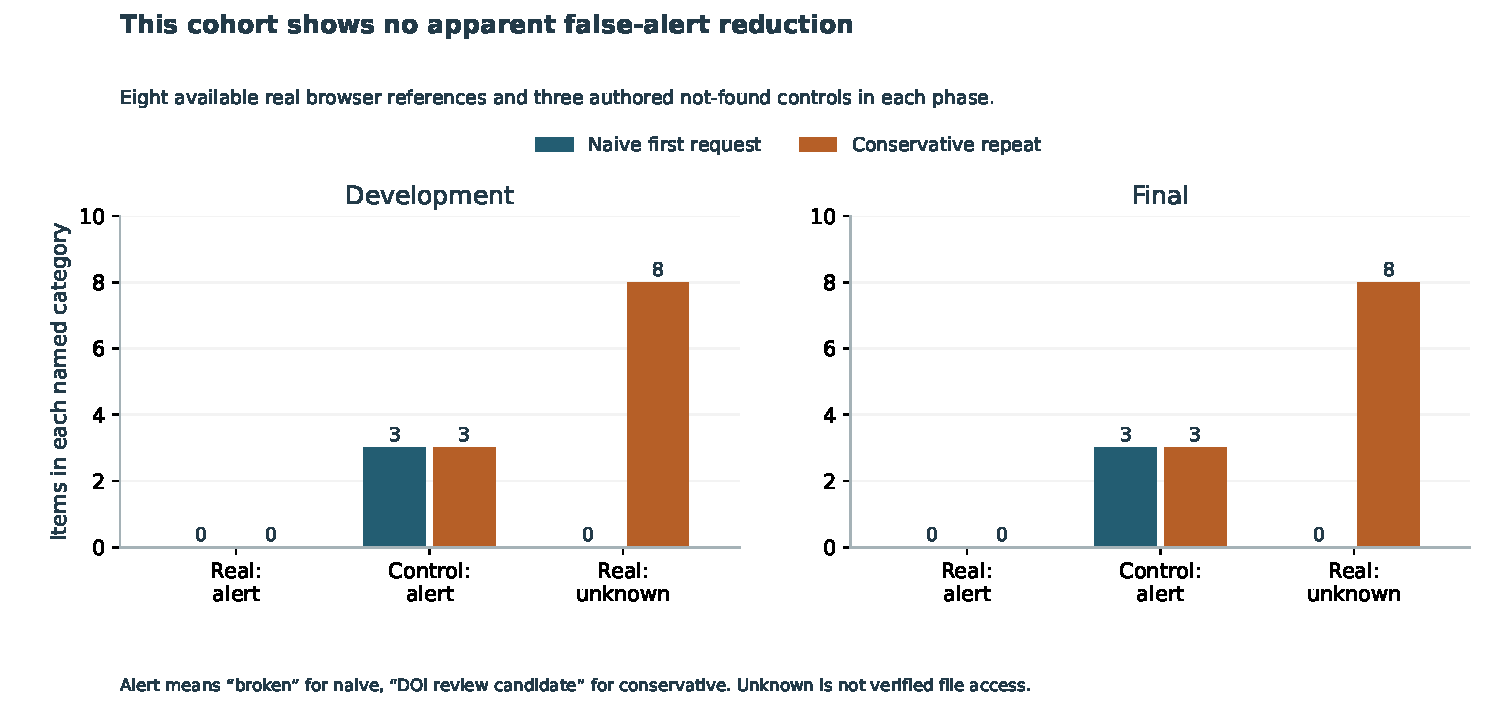
\includegraphics[width=\linewidth]{images/conditional_comparison.pdf}\end{center}

Each phase has \MDevReal{} available real references and \MDevControls{} observed not-found controls. Both rules produce three control alerts and zero apparent false alerts. Conservative unknowns stay explicit; binary non-alert counts do not certify accessible data. Conditional precision/recall denominators concern this authored mixture, rather than genuinely missing scholarly datasets.

Source, rule/checker, complete development evidence and the offline exercise are committed in \MDeps{} dependency hashes before any final landing/reference inspection. Final uses other parent/target DOI groups, while sharing a platform and possible semantic dependence. It repeats the negative comparison without rule changes or reference-driven reselection.
\newpage
\section*{4. References and repeats are not simultaneous truth}
References are captured separately from rule output. Available requires visible dataset context matching the source DOI; status alone is insufficient. Controls require a matching visible not-found result. Agent inspection is not independent human validation; browser/probe paths may share service backends.

\begin{center}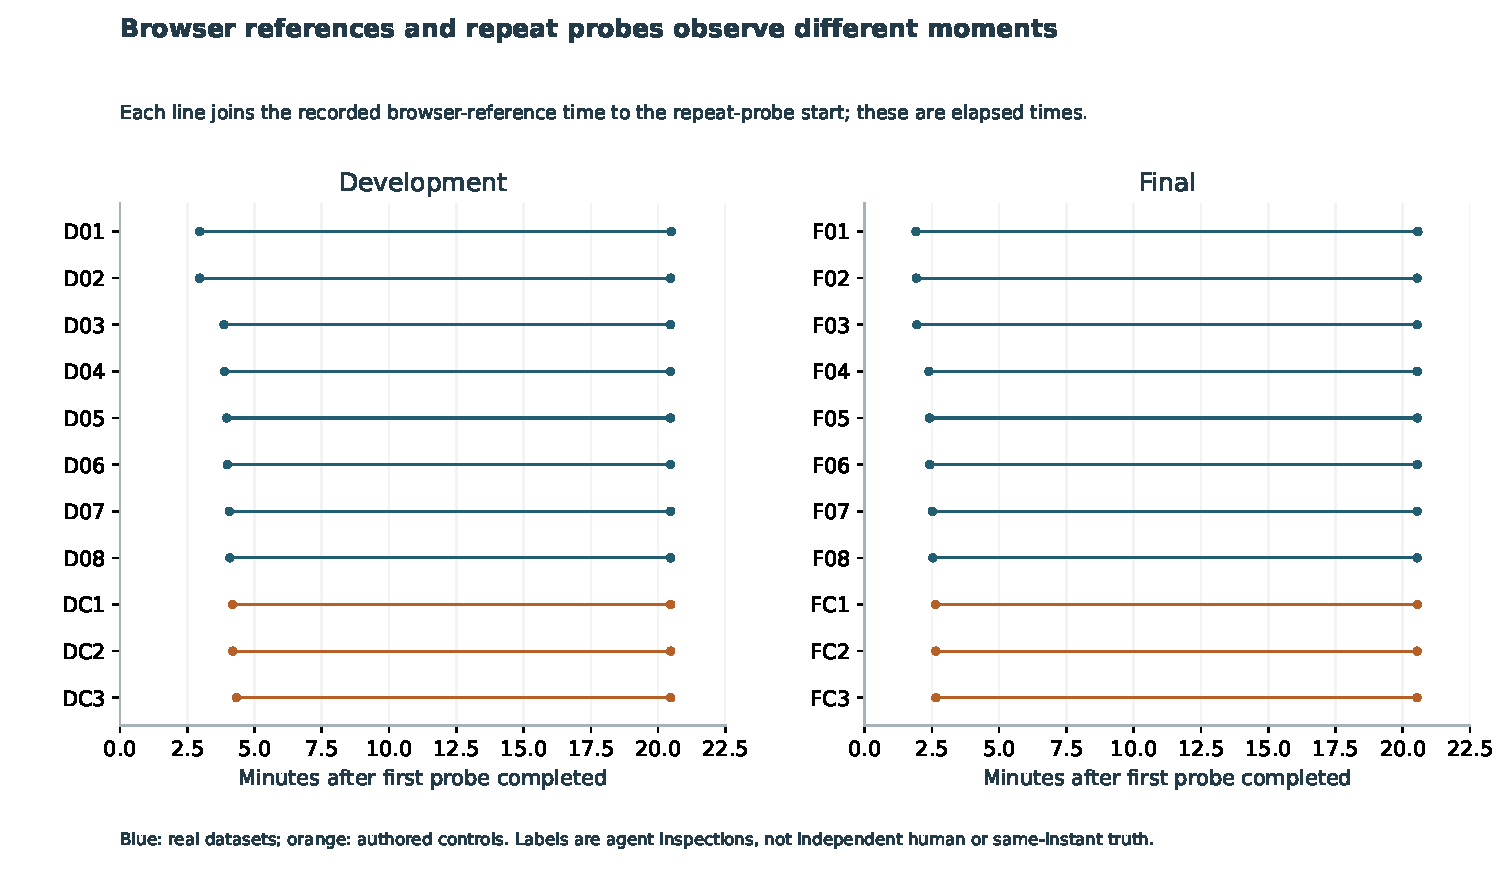
\includegraphics[width=\linewidth]{images/observation_timing.pdf}\end{center}

Per-item repeat gaps range from \MDevRepeatMin{} to \MDevRepeatMax{} seconds in development and \MFinalRepeatMin{} to \MFinalRepeatMax{} in final. Reference times are \MDevReferenceMin{}--\MDevReferenceMax{} seconds after first development probes and \MFinalReferenceMin{}--\MFinalReferenceMax{} seconds after first final probes. These are elapsed intervals, not error bars or same-instant ground truth.

The evidence gate requires four available real pages and all three observed controls per phase; all eight real pages and three controls meet it here. Unknown references would remain outside binary metrics. A short repeat interval establishes neither permanence nor long-term reliability.

A stronger next study should add representative repositories, genuinely unresolved published identifiers and independent task-specific adjudication. Usable-data decisions need separate authorized file-access, source-rights and scientific-support checks.
\newpage
\section*{5. Reproduce bounded evidence, then interpret it}
Native original/transcript/DOM, chronology, action and denominator checks pass \MDevChecks{} development and \MFinalChecks{} final conditions. Thirty-six fixture methods cover DOI representations, redirect/credential/private-host guards, 202/204/403/404/410/429/5xx, early/missing repeats, Retry-After, truncated HTML, unavailable references and zero denominators. These finite checks do not establish a universal detector.

Three inspected figures pass \MFigureValues{} source-value and \MCoordinates{} actual SVG-coordinate checks, with nine hashes. A synthetic-signature fixture stopped the first staged scan; the original and failed receipt remain private. A generic explicitly invalid signature preserves the rejection check. The scanner and real source evidence remain unchanged. A non-secret file-selector query was removed from one public reference URL before freeze, preserving its DOM, time and label.

\begin{verbatim}
python -m unittest discover -s tests -v
python src/freeze_proof.py
python src/replay.py --output ../fresh-replay
python src/triage_cli.py examples/repeated-not-found.json
python src/verify_figures.py
\end{verbatim}
The CLI reads captured or authored observations offline, keeps file access untested and sends no maintainer message. Use a fresh replay output outside a full-history checkout. Release also requires isolated runtime checks, frozen/source hashes, source-bound PDF displays/pages, scoped publication audit and exact candidate/main CI, matching content and an annotated tag.

\section*{Primary sources and prior work}
\small
Crossref. REST API, filters and relationships. \url{https://www.crossref.org/documentation/retrieve-metadata/rest-api/}. Deposited links are assertions.

DataCite. Public REST API and metadata harvesting. \url{https://support.datacite.org/docs/rest-api}; \url{https://support.datacite.org/docs/harvesting-datacite-doi-metadata}. Public Findable scope and CC0 metadata do not license underlying files.

IETF. RFC 9110, HTTP Semantics, section 15.3.3. \url{https://www.rfc-editor.org/rfc/rfc9110.html}. Accepted requests do not establish completed content.

Klein et al.(2014). Reference-rot research. \url{https://doi.org/10.1371/journal.pone.0115253}. Historical rates are not assumed current. No new detector or scientific-priority claim.

\normalsize\textbf{Publication scope.} This independent manuscript is eligible for the reviewed GitHub subset. Formal-publication projects, including Azure optimization, remain private. Clinical, deployment, adoption, automatic-repair and realized-benefit outcomes are unmeasured.
\end{document}
